\documentclass[12pt]{article}

\usepackage[utf8]{inputenc}
\usepackage{amsmath}
\usepackage{amssymb}
\usepackage{graphicx}
\usepackage{hyperref}
\usepackage{geometry}
\usepackage{tikz}
\usetikzlibrary{shapes.geometric, arrows.meta, positioning, shadows}
\usetikzlibrary{positioning}
\geometry{a4paper, margin=1in}


\begin{document}

\section*{Structure}
I will start by discussing the points mentioned in the Emails (see Section~\ref{sec:email-points}), then 
I will start by describing the overall approach I discussed in Thursday's meeting. And while doing so, relating it to the points raised by Prof. Monni and Ahmad (see Section~\ref{sec:approach}).  After that I will propose the tasks division (see Section~\ref{sec:tasks}).

\section{Discussing Email Points}
\label{sec:email-points}
\begin{itemize}
  \item Yes we are on the same page that each $K_{(i,j)}^{(k)} = K^{(k)}(f^{(k)}(x_i^{(k)}), f^{(k)}(x_j^{(k)}))$ where $f^{(k)}$ is non linear mapping of the $k$'th feature space. And then to get the entry $K_{(i,j)}= \sum_{k=1}^{p} \alpha_k K_{(i,j)}^{(k)}$. This $\alpha_k$ is what ahmad was referring as the weight associated with each kernel, where with training some of them might go to zero, \textbf{IF WE USE appropriate methods to do so} (one example is using L1 regularization on the weights $\alpha_k$, similar to how in linear regression with a lasso penalty some of the weights of the features can go to zero), and so we can start using our architecture to as a feature selection algorithm. I need to emphasize the point that at before taking any step in our Optimization procedure, we need to compute the Gram matrix $K$ using the current values of the weights $\alpha_k$ and the current hyperparameters of each kernel $K^{(k)}$, this to ensure that $K_{(i,j)}$ is the same global mapping $\forall (i,j)$, notice how from this construciton we are guarrantying that also $f^{(k)}$ is the same $\forall (i,j)$ within the $k$'th feature space. In our presentation we need to emphaize this point
  \item Notice how while constructing $K$ we can only construct $K_{(i,j)}$ and then set $K_{(j,i)} = K_{(i,j)}$ as mayssa and prof monni pointed out. 
  \item Now regarding the point about adding a jitter term to the diagonal of $K$, this to ensure numerical stability especially in pytorch where we will be inverting $K$. BUT I am interested about knowing this point that professor monni mentioned and I quote ``Notice that adding instead a positive  number
K(i,j)=K(i,j)+epsilon for all i, j need not lift the eigenvalues from zero to positive.'' I noticed that numerically it is true, but why is true mathematically? I would like to understand this point better. I understood adding a jitter but why only on the diagonal?
  \item Regarding the PCA point made by ahmad, I liked the idea of it, I think this might be an innovation in the field. I think for experimentation purposes (i.e. what we would be presenting saturday, we can mention it as a future work), in my opininon focusing now on getting something working first is more important. Also I do not think there is a need to compare what we did with other methods, in my opinion focusing now on toy models and presenting these on saturday is more important. 
  \item Another question I have Professor Monni Mentionned ``$y_i=x_i + \epsilon_i$ is more difficult than havig the toy model $y_i = f(x_i) + \epsilon_i$''
  \item I think the point of interpretaibility is very nice, we can even show the graphs in the presentation, but I think this is not a trivial point to make, because we need to construct appropriate toy models to illustrate this point well. 
\end{itemize}

\section{Overall Approach: Gaussian Processes and Bayesian Optimization}
\label{sec:approach}
In my approach I will try to focus on two things: \ref{sec:gp-setup}training kernels in the setup of Gaussian processes, and the second one \ref{sec:mitigating-kernels} the point that Ahmad raised (in section 3.1 of his email) ``Can our kernel imitate known kernels? ''
\subsection{Guassian Processes Setup}
\label{sec:gp-setup}
So here I will describe the generation process(we are nature) and then the training process (we are the scientists trying to learn given these data only).
\subsubsection*{Generating the Data (Nature)}
In my setup I will assume that the data is generated as follows: 
\[
y = f(x) + \epsilon , \quad \epsilon \sim \mathcal{N}(0, \sigma^2)
\]
I will generate the matrix $X$ with $n$ samples and $p$ features. (I will use a small $p$ like professor monni suggested, around 5 to 10) and $\sigma_2$ to be small to have a high signal to noise ratio. (side note after training is done we can draw a graph of the loss vs different values of SNR to show how the model degrades with increasing noise). The generation of $X$ can be done using a mv or even any other distribution, because the disrbution that we really care about is the one of $f(x)$ which will be in my toy model a multivariate normal distribution with a known kernel $K_{true}$ and mean zero. Why I chose a mv for $f(x)$ because I want the assumption of GP (in training) to be actually true. Later one we can try and violate this. \textbf{Formal Setup:}\\
Let $X = [x_1, x_2, \ldots, x_n]^T$ be the input data matrix where each $x_i \in \mathbb{R}^p$. We assume that the function values $f = [f(x_1), f(x_2), \ldots, f(x_n)]^T$ are drawn from a multivariate normal distribution:
\[f \sim \mathcal{N}(0, K_{true})\]
where $K_{true}$ is the true kernel matrix defined by a known kernel function (RBF, linear, ...) evaluated at the input points.  More specifically, the entries of $K_{true}$ are given by:
\[K_{true}(i,j) = k_{true}(x_i, x_j)\]
for a chosen kernel function $k_{true}$. Again $k_{true}$ must be the SAME kernel $\forall (i,j)$. \\ \\
Now that we have the function values $f$, the observed outputs $y$ are then generated by adding Gaussian noise to the function values:
\[y_i = f_i + \epsilon_i, \quad \epsilon_i \sim \mathcal{N}(0, \sigma^2)\]
where $\sigma^2$ is the noise variance (a small value to ensure high SNR for now).

\subsubsection*{Training the Model (Scientists)}
In the training phase, we will assume a Gaussian process prior over the function $f(x)$ with a kernel $K$ that is a weighted sum of multiple kernels as discussed earlier:
\[K(x_i, x_j) = \sum_{k=1}^{p} \alpha_k K^{(k)}(f^{(k)}(x_i^{(k)}), f^{(k)}(x_j^{(k)}))\]

For now I will assume always that $\alpha_k=1$ (i.e. not trainable parametrs, future experiments i will start including them as trainable (relating back to the feature selection point made earlier)). The only trainable parameters will be the hyperparameters of each kernel $K^{(k)}$ (also for now the $f^{(k)}$ will be the identity function). The training objective will be to maximize the log marginal likelihood of the observed data $y$ given the inputs $X$ (given by equation 4 in NKN paper):
\[
\operatorname*{argmax}_{\theta} -\frac{1}{2} y^T (K + \sigma^2 I)^{-1} y - \frac{1}{2} \log |K + \sigma^2 I| - \frac{n}{2} \log 2\pi
\]

where $\theta$ represents the hyperparameters of the kernels and $\sigma^2$ is the noise variance. I will use ggraident descent no fancy optimizers for now to optimize this objective with respect to the hyperparameters $\theta$.
\begin{itemize}
  \item \textbf{Question:} In the training do I include the true value of $\sigma^2$ used in the data generation or do I treat it as a hyperparameter to be learned as well? Or not account for it so directly in the model? (i.e. just use $K$ instead of $K + \sigma^2 I$ in the above equation)
\end{itemize}
Again here while training I will keep on observing the eiegenvalues of $K$ to ensure numerical stability, and add jitter to the diagonal if needed. \\ 

After training is done I will compare the learned kernel matrix $K$ with the true kernel matrix $K_{true}$ used in data generation using appropriate metrics (Frobenius norm, MSE ...etc). This will help us assess how well our model has learned the underlying kernel structure of the data. 
\subsection{Mitigating other Kernels}
\label{sec:mitigating-kernels}
This is what ahmad raised in his email (section 3.1), and similar to the first dummy example I introduced in Thursday's meeting, in Thursday's meeting I was trying to replicate a linear kernel, I will extend this to more sohpisticated kernels like RBF, periodic ...etc. Back then I was using the MSE between the true kernel matrix and the learned kernel matrix as a loss function to optimize the hyperparameters of the kernels in the weighted sum. I can now incorporate the loss that Professor Monni suggested (fobenius norm between the two kernel matrices). \textbf{Formal Setup:} \\
The setup here will be slightly different than before. Because now the input data will be of $n^2$ samples (each sample corresponds to a pair $(x_i, x_j)$ from the original data), and the output will be the corresponding entries of the true kernel matrix $K_{true}(i,j)$. So the input data matrix will be:
\[X_{pairs} = [(x_1, x_1), (x_1, x_2), \ldots, (x_n, x_n)]^T\]
with $n^2$ samples, and the output vector will be:
\[y_{kernel} = [K_{true}(1,1), K_{true}(1,2), \ldots, K_{true}(n,n)]^T\]
The model will then learn to predict the kernel values using the weighted sum of kernels as before(but again here for now I wil l keep $\alpha_k=1$ and only train the hyperparameters of each kernel, also for now the $f^{(k)}$ will be the identity function). So the learned kernel matrix entries will be:
\[K_{learned}(x_i, x_j) = \sum_{k=1}^{p} \alpha_k K^{(k)}(f^{(k)}(x_i^{(k)}), f^{(k)}(x_j^{(k)}))\]
The training objective will be to minimize the Frobenius norm between the learned kernel matrix $K_{learned}$ and the true kernel matrix $K_{true}$ , or the MSE between the corresponding entries:
\[\operatorname*{argmin}_{\theta} \|K_{learned} - K_{true}\|_F^2\]
where $\theta$ represents the hyperparameters of the kernels. Again I will use gradient descent to optimize this objective. \\
\section{Task Division}
\label{sec:tasks}
This is my proposed task division (waiting for your feedback), and we can meet on \textbf{Monday to discuss the progess of each of us.} \\
Mayssa will focus on the interpretability aspect (point 3 mentioned in Section 3 of Ahmad's email).  
Ahmad will continue working on the classification setup (point 2 mentioned in Section 3 of Ahmad's email).  
I will handle point 1 from Section 3 of Ahmad's email, incorporating it into the Gaussian process setup discussed earlier in Section~\ref{sec:approach}.
\newpage 

\[
p_{Y|X}(\mathbf{y}| \mathbf{x}) = \frac{1}{(2\pi)^{n/2} |\Sigma|^{1/2}} \exp\left(-\frac{1}{2}(\mathbf{y} - \boldsymbol{\mu})^T \Sigma^{-1} (\mathbf{y} - \boldsymbol{\mu})\right) , \quad \mathbf{y} \in \mathbb{R}^n
\]
The univariate guassian normal in y is given by, using first the sim: 
\newpage
$y \sim \mathcal{N}(\mu, \sigma^2), \quad p_{Y}(y) = \frac{1}{\sqrt{2\pi \sigma^2}} \exp\left(-\frac{(y - \mu)^2}{2\sigma^2}\right) , \quad y \in \mathbb{R}$
\newpage
Now for the multivariate case: \newpage
$\mathbf{y} \sim \mathcal{N}(\boldsymbol{\mu}, \Sigma) ,  \quad \mathbf{y} \in \mathbb{R}^n$

\newpage
Liken in any machine learning we have the setyp of a set of data points: 
\newpage
dfsdhf\\
$D = \{(\mathbf{x}_i, y_i)\}_{i=1}^n \quad \mathbf{x}_i \in \mathbb{R}^p , \quad y_i \in \mathbb{R}$\\
$y = f(\mathbf{x}) + \epsilon, \quad \epsilon \sim \mathcal{N}(0, \sigma^2)$\\

\newpage
sdfsdfd\\\\
$\mathbf{f}|\mathbf{X} \sim \mathcal{N}(\textbf{0}, \mathcal{K}_{\mathbf{X}\mathbf{X}}) \implies  \mathbf{Y}|\mathbf{X} \sim \mathcal{N}(\mathbf{0},   \mathcal{K}_{\mathbf{X}\mathbf{X}} +\sigma^2\mathbf{I}) $ \newpage
Fix a Kernel(e.g. RBF):  $ K(\mathbf{x}_i, \mathbf{x}_j) = \exp\left(-\frac{||\mathbf{x}_i - \mathbf{x}_j||^2}{2\rho^2}\right) \quad \forall i,j$ \newpage
$O(n^3)$ \newpage

$\max\limits_{K_{\mathbf{x}\mathbf{x}}} \ \  p(\textbf{y}|\mathbf{x}; K_{\mathbf{x}\mathbf{x}})$ 
\newpage

$ \hat{K} \quad \hat{K}(\mathbf{x}_i, \mathbf{x}_j) \quad \forall i,j \quad $
\newpage
$p(\textbf{y}|\mathbf{x}; \hat{K})$
\newpage 
$\mathbf{x_*} \in \mathbb{R}^p$ \newpage 
$K^{true}$ \newpage 
$K^{obs}= K^{true} + \mathcal{E}, \quad \mathcal{E} \sim \mathcal{N}(\textbf{0}, \sigma^2\textbf{I})$ \newpage
$ \text{Frobenius: }\min\limits_{K} \ \  ||K^{obs} - K||_F^2 , \quad \text{MSE: } \min\limits_{K} \ \  \frac{1}{n^2}||K^{obs} - K||^2 $ 
\newpage
$D = \{\mathbf{x}_i\}_{i=1}^n \quad \mathbf{x}_i \in \mathbb{R}^p$ 
\newpage 
\begin{tikzpicture}[
    node distance=1.8cm,
    every node/.style={font=\small},
    box/.style={draw, rectangle, minimum width=2.7cm, minimum height=1.2cm, align=center}
]

% Pair (i,j)
\node[box] (pair) {All pairs\\$(\mathbf{x}_i,\mathbf{x}_j)$};

% Network
\node[box, right=3cm of pair] (net) {Our Network};

% Single K_ij output
\node[box, right=2.6cm of net, minimum width=1.7cm] (Kij) {$\hat{K}_{ij}$};

% Matrix assembly
\node[box, below=1.5cm of Kij] (matrix) {$\hat{K}\in\mathbb{R}^{n\times n}$};

% Loss
\node[box, left=3cm of matrix] (loss) {$\ell\!\left(K^{\text{true}},\,\hat{K}\right)$};

% Backprop block (boxed)
\node[box, below=1.2cm of loss, minimum width=2.3cm] (bpbox) {Backpropagation};

% Arrow label (not boxed)
% \node[below=0.4cm of loss] (bplabel) {backpropagate};

% Arrows forward
\draw[->] (pair) -- node[midway,above]{$ \forall \ (i,j)$} (net);
\draw[->] (net) -- (Kij);
\draw[->] (Kij) -- node[right]{fill matrix} (matrix);
\draw[->] (matrix) -- (loss);

% Backprop arrow
\draw[->] (loss) -- (bpbox);

\end{tikzpicture}
\newpage
\(K^{\text{true}}(\mathbf{x}_i,\mathbf{x}_j)
= K^{\text{true}}(\mathbf{x}_i^{(0:m)},\,\mathbf{x}_j^{(0:m)}) ,\quad m<p \quad \quad \text{where we are given } \mathbf{x} \in \mathbb{R}^p\)




\newpage 

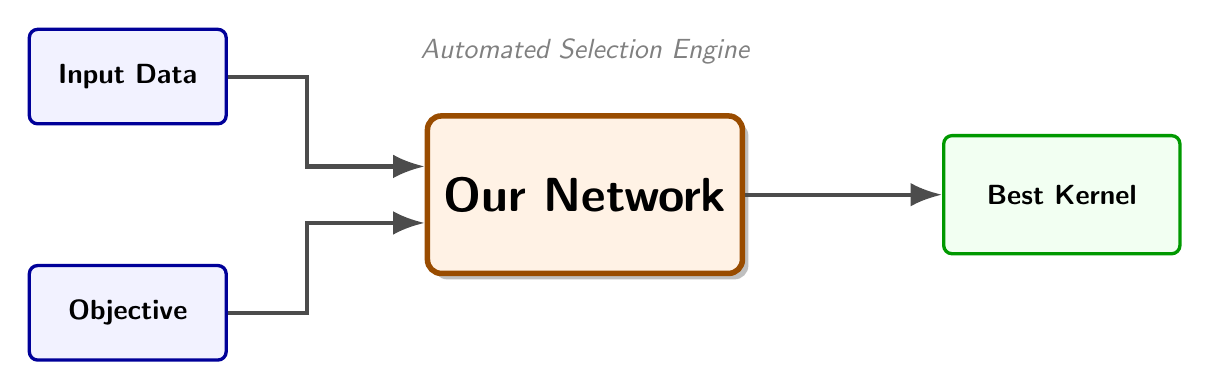
\begin{tikzpicture}[
    % Define standard styles for the diagram components
    node distance=2.5cm,
    inputnode/.style={
        rectangle,
        draw=blue!60!black,
        fill=blue!5,
        very thick,
        minimum width=2.5cm,
        minimum height=1.2cm,
        align=center,
        rounded corners=3pt,
        font=\sffamily\bfseries
    },
    processnode/.style={
        rectangle,
        draw=orange!60!black,
        fill=orange!10,
        line width=2pt,
        minimum width=4cm,
        minimum height=2cm,
        align=center,
        rounded corners=5pt,
        drop shadow,
        font=\sffamily\LARGE\bfseries
    },
    outputnode/.style={
        rectangle,
        draw=green!60!black,
        fill=green!5,
        very thick,
        minimum width=3cm,
        minimum height=1.5cm,
        align=center,
        rounded corners=3pt,
        font=\sffamily\bfseries
    },
    arrow/.style={
        -{Latex[length=4mm, width=3mm]},
        line width=1.5pt,
        draw=gray!60!black
    }
]

% --- Nodes ---

% Central Process (The Package)
\node[processnode] (package) {Our Network};

% Inputs (positioned relative to the center)
\node[inputnode, left=of package, yshift=1.5cm] (data) {Input Data};
\node[inputnode, left=of package, yshift=-1.5cm] (obj) {Objective};

% Output
\node[outputnode, right=of package] (kernel) {Best Kernel};

% --- Connections ---
% Drawing arrows with flowing paths
\draw[arrow] (data.east) -- + (1,0) |- (package.170);
\draw[arrow] (obj.east)  -- + (1,0) |- (package.190);
\draw[arrow] (package.east) -- (kernel.west);

% Optional: Add a "Ready to Use" label above
\node[above=0.5cm of package, font=\sffamily\itshape\color{gray}] {Automated Selection Engine};

\end{tikzpicture}

\newpage 
\[
f \sim \mathcal{GP}\!\left(0,\, k(\cdot,\cdot)\right),
\]
\[
\mathbf{f} = (f(\mathbf{x}_1),\ldots,f(\mathbf{x}_n))^T 
\sim \mathcal{N}\!\left(\mathbf{0},\, K_{\mathbf{X}\mathbf{X}}\right).
\]
\newpage 
$\max\limits_{k_{\theta}} \ \  \log \ p(\textbf{y}|\mathbf{x}; K_{\mathbf{x}\mathbf{x}})$
\newpage
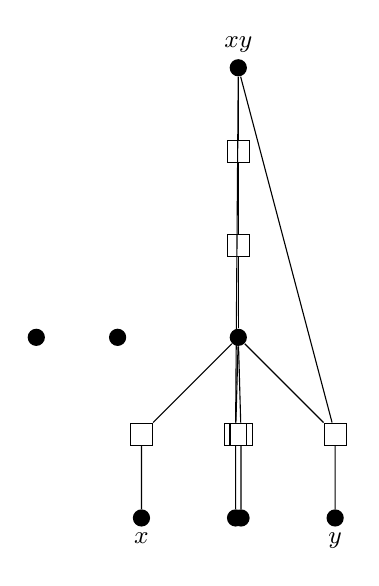
\begin{tikzpicture}[
    every node/.style={font=\small},
    dot/.style={circle,fill=black,inner sep=2.2pt},
    sq/.style={draw,rectangle,minimum size=8pt}
]

% Top
\node[dot] (xy) {};

% Middle column
\node[sq, below=0.8cm of xy] (sq1) {};
\node[sq, below=0.9cm of sq1] (sq2) {};
\node[dot, below=0.9cm of sq2] (mid) {};

% Left branch from mid
\node[sq, below left=1.0cm and 1.0cm of mid] (L1) {};
\node[sq, right=0.9cm of L1] (L2) {};
\node[dot, below=0.8cm of L1] (x) {};
\node[dot, below=0.8cm of L2] (x2) {}; % small neighbor dot

% Right branch from mid
\node[sq, below right=1.0cm and 1.0cm of mid] (R1) {};
\node[sq, left=0.9cm of R1] (R2) {};
\node[dot, below=0.8cm of R1] (y) {};
\node[dot, below=0.8cm of R2] (y2) {}; % small neighbor dot

% Extra isolated dots (left side)
\node[dot, left=1.3cm of mid] (is1) {};
\node[dot, left=0.8cm of is1] (is2) {};

% Connections (vertical)
\draw (xy) -- (sq1) -- (sq2) -- (mid);

% Left Branch connections
\draw (mid) -- (L1) -- (x);
\draw (mid) -- (L2) -- (x2);

% Right Branch connections
\draw (mid) -- (R1) -- (y);
\draw (mid) -- (R2) -- (y2);

% Top diagonal branches
\draw (xy) -- (R1);
\draw (xy) -- (L2);

% Labels
\node[below=2pt] at (x) {$x$};
\node[below=2pt] at (y) {$y$};
\node[above=2pt] at (xy) {$xy$};

\end{tikzpicture}
\newpage
\begin{tikzpicture}[
    dot/.style={circle, fill=black, inner sep=1.5pt},
    gate/.style={rectangle, draw, minimum size=6mm},
    >=stealth
]

% Define the nodes
% Input nodes
\node[dot, label=below:$x$] (x) at (0, 0) {};
\node[dot, label=below:$y$] (y) at (5, 0) {};

% Intermediate layer 1 (Gates)
\node[gate] (gate1) at (0, 2) {$\setminus$}; % Simulating the left-leaning curve
\node[gate] (gate2) at (1.5, 2) {$\cup$}; % Simulating the upward-facing curve
\node[gate] (gate3) at (3.5, 2) {$\setminus$}; % Simulating the left-leaning curve
\node[gate] (gate4) at (5, 2) {$\cup$}; % Simulating the upward-facing curve

% Intermediate layer 2 (Dots/Junctions)
\node[dot] (mid1) at (1.5, 4) {};
\node[dot] (mid2) at (3.5, 4) {};

% Mid-level nodes (for spacing and the ellipses in the original image)
\node[dot] at (-1.5, 4) {};
\node[dot] at (-0.5, 4) {};
\node at (0.5, 4) {$\dots$}; % For the missing dots/lines on the left
\node at (2.5, 4) {$\dots$}; % For the missing dots/lines in the middle

% Intermediate layer 3 (Gates)
\node[gate] (gate5) at (1.5, 6) {$\cup$}; % Simulating the upward-facing curve
\node[gate] (gate6) at (3.5, 6) {$\setminus$}; % Simulating the left-leaning curve

% Output node
\node[dot, label=above:$xy$] (xy) at (2.5, 8) {};

% --- Draw the connections (Lines) ---

% From x and y to Gate Layer 1
\draw (x) -- (gate1);
\draw (x) -- (gate2); % Connecting x to gate2
\draw (y) -- (gate3); % Connecting y to gate3
\draw (y) -- (gate4);

% From Gate Layer 1 to Junction Layer 2
\draw (gate1) -- (mid1);
\draw (gate2) -- (mid1);
\draw (gate3) -- (mid2);
\draw (gate4) -- (mid2);

% Connections between Junction Layer 2 nodes
\draw (mid1) -- (gate5);
\draw (mid1) -- (gate6);
\draw (mid2) -- (gate5); % Connecting mid2 to gate5

% Connections from Junction Layer 2 to Output Layer 3 (and possibly other nodes)
\draw (mid1) -- (gate5);
\draw (mid2) -- (gate6);
\draw (mid2) -- (gate4); % Looks like mid2 connects to gate4 in the original image

% From Gate Layer 3 to Output
\draw (gate5) -- (xy);
\draw (gate6) -- (xy);

% Add the "multiplication" label
\node[anchor=west] at (-2.5, 8) {\textbf{(a) multiplication}};

\end{tikzpicture}
\end{document}